% ---------------------------------------------------------------------------
% Author guideline and sample document for EG publication using LaTeX2e input
% D.Fellner, v1.13, Jul 31, 2008

\documentclass{egpubl}
\usepackage{pg2016}

% --- for  Annual CONFERENCE
% \ConferenceSubmission % uncomment for Conference submission
% \ConferencePaper      % uncomment for (final) Conference Paper
% \STAR                 % uncomment for STAR contribution
% \Tutorial             % uncomment for Tutorial contribution
% \ShortPresentation    % uncomment for (final) Short Conference Presentation
%
% --- for  CGF Journal
% \JournalSubmission    % uncomment for submission to Computer Graphics Forum
% \JournalPaper         % uncomment for final version of Journal Paper
%
% --- for  CGF Journal: special issue
 \SpecialIssueSubmission    % uncomment for submission to Computer Graphics Forum, special issue
% \SpecialIssuePaper         % uncomment for final version of Journal Paper, special issue
%
% --- for  EG Workshop Proceedings
% \WsSubmission    % uncomment for submission to EG Workshop
% \WsPaper         % uncomment for final version of EG Workshop contribution
%
 \electronicVersion % can be used both for the printed and electronic version

% !! *please* don't change anything above
% !! unless you REALLY know what you are doing
% ------------------------------------------------------------------------

% for including postscript figures
% mind: package option 'draft' will replace PS figure by a filename within a frame
\ifpdf \usepackage[pdftex]{graphicx} \pdfcompresslevel=9
\else \usepackage[dvips]{graphicx} \fi

\PrintedOrElectronic

% prepare for electronic version of your document
\usepackage{t1enc,dfadobe}

\usepackage{egweblnk}
\usepackage{cite}


\usepackage{balance}  % to better equalize the last page
\usepackage{graphics} % for EPS, load graphicx instead
\usepackage{times}    % comment if you want LaTeX's default font
\usepackage{url}      % llt: nicely formatted URLs


\newcommand\tabhead[1]{\small\textbf{#1}}

\usepackage{customized_commands}

% For backwards compatibility to old LaTeX type font selection.
% Uncomment if your document adheres to LaTeX2e recommendations.
% \let\rm=\rmfamily    \let\sf=\sffamily    \let\tt=\ttfamily
% \let\it=\itshape     \let\sl=\slshape     \let\sc=\scshape
% \let\bf=\bfseries

% end of prologue

% ---------------------------------------------------------------------
% EG author guidelines plus sample file for EG publication using LaTeX2e input
% D.Fellner, v1.17, Sep 23, 2010


\title[Toward Support-free 3D Printing:]%
      {Toward Support-free 3D Printing: A skeletal Approach for Partitioning Models}

% for anonymous conference submission please enter your SUBMISSION ID
% instead of the author's name (and leave the affiliation blank) !!
\author[1017]{1017}

%\author[D. Fellner \& S. Behnke]
%       {D.\,W. Fellner\thanks{Chairman Eurographics Publications Board}$^{1,2}$
%        and S. Behnke$^{2}$
%%        S. Spencer$^2$\thanks{Chairman Siggraph Publications Board}
%        \\
%% For Computer Graphics Forum: Please use the abbreviation of your first name.
%         $^1$TU Darmstadt \& Fraunhofer IGD, Germany\\
%         $^2$Institut f{\"u}r ComputerGraphik \& Wissensvisualisierung, TU Graz, Austria
%%        $^2$ Another Department to illustrate the use in papers from authors
%%             with different affiliations
%       }

% ------------------------------------------------------------------------

% if the Editors-in-Chief have given you the data, you may uncomment
% the following five lines and insert it here
%
% \volume{27}   % the volume in which the issue will be published;
% \issue{1}     % the issue number of the publication
% \pStartPage{1}      % set starting page


%-------------------------------------------------------------------------
\begin{document}

% \teaser{
%  \includegraphics[width=\linewidth]{eg_new}
%  \centering
%   \caption{New EG Logo}
% \label{fig:teaser}
% }

\maketitle

\begin{abstract}
   We propose an algorithm for partitioning a 3D model into the least number of parts for 3D printing without using any support structure. Minimizing support structures is crucial in reducing 3D printing material and time, partition-based methods are efficient means in realizing this objective. However, any partition will inevitably induce seams and cracks on the assembled model, which affects the aesthetics and strength of the finished surface. To achieve support-free fabrication while minimizing the effect of the seams, we put forward an optimization system with the minimization of the number of partitioned components and the total length of the cuts, under the constraints of support-free printing angle, gravitational and the dimension of each part with respect to the printing dimension. We show that the optimization problem is NP-hard and propose a Monte Carlo method based on training-and-learning data to find an optimal solution to the objectives. We applied our partition method on a number of various 3D models. Finally, we validate our method by carrying out a serial of 3D printing experiments.


\begin{classification} % according to http://www.acm.org/class/1998/
\CCScat{Computer Graphics}{I.3.3}{Picture/Image Generation}{Line and curve generation}
\end{classification}

\end{abstract}





%-------------------------------------------------------------------------
\section{Introduction}

3D printing, or additive manufacturing, has drawn growing interests from researchers in computer graphics. Fused deposition modeling (FDM), stereolithographic (SLA), Selective Laser Melting (SLM) and Selective Laser Sintering (SLS) and the four most popular means of 3D printing techniques. Although 3D printing has seen its applications in producing arbitrarily intricate 3D models, the price of the printing materials, especially for those with high quality, are still outrageously high. Therefore, it is desirable to reduce materials used in the fabrication process. Note that this is also a critical operation for reducing production time and therefore the total production cost. For this purpose, an efficient method is the minimizing of support structures, which are removed in the post-processing phase of the fabrication task.

As for minimizing support structures, Autodesk R MeshMixerTM provides a semiautomatic orientation optimization tool to minimize support volume, support area, structural strength, or a combination of these three attributes. However, it requires the operators�� experience in setting the geometric parameters manually. A number of literatures have studied various factors that influence the volume of supports, e.g., optimizing the topology of the support structure \cite{DumasHL14,VanekGB14}, determining an optimal fabrication direction \cite{Zhang:2015,HildebrandBA13,padhye2011multi}; partitioning any given model into a set of separate parts that preserve nice geometric features \cite{VanekGBMCSM14,SongFLF15}.

However, the partition results of these methods do not simultaneously respect the geometric features and support-free printability of the portioned parts. Further, no existing algorithms ever consider the problem of partitioning a model into the least number of pieces whose fabrication is free of support structures. The least number of portioned parts corresponds to the least number of seams on the final assembled model, which means a nice aesthetics preservation of the model surface; and the support-free fabrication means saving material to the most extent, which is very meaningful in reducing fabrication cost since the prices of printing materials (metal powder, resin, nice plastics, etc.) are still outrageously high. This motivates us to explore an efficient algorithm for solving the issue.
Our solution of the problem draws inspiration from the skeleton of organic models: the topology changes of a natural model can be determined by its skeleton, and each chunk of a mesh corresponding to a segment of the skeleton; further, the mesh chunk is a cylinder-like shape which can be printed free of support structures if the printing direction is parallel to the skeleton.

Automatically partitioning 3D models into components that are consistent with human perception is an extremely intricate due to the lack of semantic information. Therefore, we restrict our focus on organic or man-made models whose shapes are well-defined by their skeletons. Further, support structures are required for the interior and exterior surface of a mesh model during the 3D printing process. For simplicity, our approach assumes that the interior of a mesh model is fully filled, usually the infill can be set as a grid whose porosity can be varied by users, as allowed in almost all existing commercial 3D printing software. This is very useful in preserving the surface quality of any printed object. Therefore, our objective is to partition a model according to the growth of its skeleton. Formally, given a 3D printer, if a facet subtends to a common axis by an angle of less than or equal to, then the facet can be printed without using any support structure. This inspires us to compute a minimum set of subgraph of the skeleton, such that each arc in any subgraph subtends to a common axis by an angle of less than or equal to ?, the corresponding chunk of the mesh is therefore support-free as printed along this axis. In general, a cone of axes satisfies the angle constraint. However, the volume of the chunk should be within the working space of the printer. Further, if the center of mass of the chunk diverts from the support center too much, e.g., the gravitational torque applied at the mass center is too far away from the center of support that it bends the printing model by a layer of thickness, then the surface quality of the model is poor or the printing task fails since the next printing layer cannot be firmly attached to the previous layer.

Our method makes the following contributions:

\begin{itemize}
\item {We partition any given mesh model into the least number of parts that are printable free of support structures; meanwhile, we preserve the aesthetics of the surface finish with the least number of seams whose length is minimized.}
\item {We propose a partition method based on the guide of 1D Laplacian skeleton of any given mesh model.}
\end{itemize}

%-------------------------------------------------------------------------
\section{Related Work}

Our work is focused on model partition, with the particular purpose for support-free fabrication. Here we briefly review a set of most relevant recent works.

\textbf{Computational Fabrication.} Recently, an increasing body of research work has been devoted to computational fabrication using 3{D} printing as the emergence of advanced 3{D} printing devices. In computer graphics, a number of literatures have focused on the fabrication of 3{D} models using 3{D} printers. Optimization works have been devoted to structural designs with emphasis on saving printing materials while preserving certain strength \cite{StavaVBCM12,ZhouPZ13,WangWYLTTDCL13,Umetani:2013:CSA,LuSZWFCSTCC14}. The modeling of some particular features have also been studied, for example, deformation behavior \cite{SkourasTCBG13}, animated mechanical characters \cite{CorosTNSFSMB13,CeylanLMAP13}, articulated models with mobile joints \cite{BacherBJP12,CaliCAKSKW12}, models spinnable motions \cite{Bacher14}, and self-balancing \cite{PrevostWLS13}.


\textbf{Shape Decomposition.} In geometry processing, decomposing a shape into meaningful parts is a fundamental problem \cite{Kaick:2014:SSA}. Many efforts have been devoted to the problem of model decomposition. An excellent survey can be found in \cite{Shamir08}. A large body of research are focusing on partitioning a given 3{D} model into parts which agree with human perception \cite{KatzT03,KatzLT05,JiLCW06,LiuZ07,Golovinskiy:2008,ChenGF09,KaickFKAC14}, among which geometric features captures shape concaveness are mostly exploited in accordance with the minima rules \cite{hoffman1984parts,hoffman1997salience}. Other approaches are more application-oriented. For example, texture mapping techniques often require the input shape being decomposed into charts which can be flatten to match image textures \cite{zhou2004iso,Garcia:2008:IIG}. Our method of partition is based on shape skeletons. Although there have been previous work on skeleton based shape decomposition \cite{lien2006simultaneous,reniers2007skeleton,AuTCCL08}, none of them is tailored towards support-free fabrication.


\textbf{Fabrication-driven Model Partition.} A 3{D} printer cannot directly print a model whose size is larger than the printer's working space. To overcome this practical limitation, Luo et al. \cite{LuoBRM12} proposed a solution to partition a given 3D model into parts for 3D printing and then assemble the parts together. This approach has a few advantages: (i) it is cost-effective in the sense that we only need to print a replacement part for a corresponding broken part; (ii) it is convenient for storage and transportation; (iii) changing some parts of a model allows innovative designs. Along this line of research, Hao et al. \cite{hao2011efficient} partitioned a large complex model into simpler 3D printable parts by using curvature-based partitioning. Hildebrand et al. \cite{HildebrandBA13} addressed the directional bias issue in 3D printing by segmenting a 3D model into a few parts each of which is assigned an optimal printing orientation. Vanek et al. \cite{VanekGBMCSM14} reduced the time and material cost of 3D printing by hollowing a 3D model into shells and breaking them into parts, a number of parameters including the total connecting area and volume of each segment are considered during the optimization process. Song et al. \cite{SongFLF15} recently developed a novel voxelization-based approach to construct inter-locking 3D parts from a given 3D model. Without using any glue, Xin et al. \cite{XinLFWHC11} and Song et al. \cite{SongFC12} take a 3D interlocking approach to construct and connect printed 3D parts to form an object assembly. None of these methods considers the problem of support-free fabrication. Most recently, Hu et al. \cite{Hu_siga14} proposed an nice algorithm for decomposing a solid model into the least number of pyramids, each of which can be fabricated without support material. However, their algorithm is only designed for volumetric models while our algorithm aims for both shell and solid models.







%-------------------------------------------------------------------------
\section{Overview}

In nature, most organic models ubiquitously contain cylindrical parts \cite{Zhou:2015:GCD}, e.g., arms, legs, etc. Moreover, an cylindrical part can be well represented by its corresponding 1{D} skeleton. Based on this property, a chunk of a mesh model can be fabricated free of support {if all the arcs of its corresponding skeleton piece subtend to a printing direction by an angle of no large than $\theta$.} Hence, our problem becomes partitioning a given 1{D} skeleton graph into a set of subgraphs such that each subgraph merits the desirable support-free property. In the remainder of the paper, by model we mean an organic mesh model of natural life form or articulated figures preserving nice topology features of real lives.

\textbf{Choise of skeleton.} Compared to natural skeletons, the medial axis can describe the topology of a mesh model more precisely \cite{ZhangXWYTW15}. However, a medial axis of a 3D mesh model is a 2D surface which cannot be conveniently applied to describe the critical topology changes of the model. Additionally, the medial axis consists of intersecting pieces of planes and conic surfaces, presenting significant complications to algorithms that attempt to construct 3D medial axes.
Reeb graph provides a possible choice for 1D skeleton. During the generation process of any Reeb graph, the slicing direction and the position of the representative node on each slide (a connected region) seriously influence the choice of critical points and therefore generation of the Reeb graph. However, the determination of suitable slicing direction and representative nodes is an intractable problem. We resort to the $1D$ Laplacian skeleton proposed by \cite{AuTCCL08} which is extracted by shrinking the mesh model using Laplacian smoothing, such 1D Laplacian skeleton provides an excellent choice for reasonably describing the geometrical and topological variations of any 3{D} model. {\color{blue}{The 1D Laplacian Skeleton represents the models very well if the following two conditions are met: (1) each critical topological feature of the model is captured by a skeleton piece; (2) each skeleton piece represents a strip of the mesh, and a skeleton piece is small enough (the pieces are dense enough) such that no dramatic change occurs within a small strip of the mesh.

For condition (1), a portion of the mesh is not represented properly by a Laplacian Skeleton piece if it is a tinny detail that have been shrunk into a point during just a few iterations of the Laplacian smoothing process. We find that these details can usually be printed out in a support-free manner if the overhang angle is not that small (e.g., larger than 10 degrees) with respect to the building platform, and that the overhang length is within a safe distance (e.g., 1-5mm) when a nozzle jumps from one point to another. See Figure \ref{fig:spike} for an illustration. We remark that this distance is long enough to address most cases when small details are not captured by a skeleton piece: it can also be printed out by any prevailing desktop 3D printer in a support-free manner due to the cohesive and elastic forces that inherent to the plastic material itself. On the other hand,  for condition (2), we use the $1D$ Laplacian skeleton provided by the authors of \cite{AuTCCL08}, which has been shown to be capable of segmenting complicated models in a nice way. For the density of the skeleton pieces, one can always add segments into the skeleton and obtain a finer representation of a smaller strip of the mesh model. Table 2 summarizes the number of skeleton arcs used to represent the mesh models. Considering the number of critical branches of each model, the skeleton pieces are dense enough to describe the model.}


\begin{figure}[t!]
  \centering
  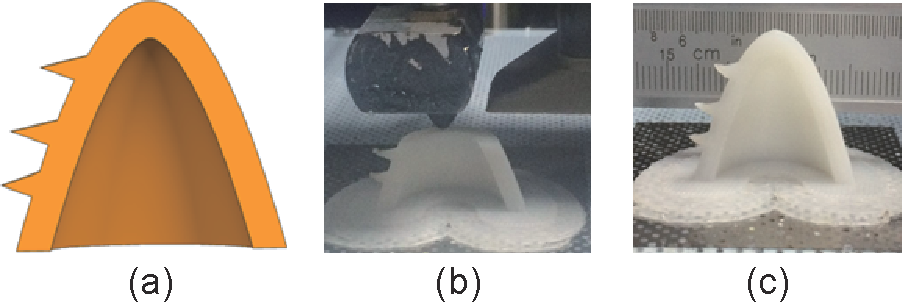
\includegraphics[width=0.7\linewidth]{figs/spike.png}
  \caption{\label{fig:spike}%
           Support-free printing of a model with some spikes on it: the length of the spikes is $4 mm$, the overhang angle is 15 degrees, the model is fabricated by a Zortrax M200 3D printer.}
\end{figure}

%Figure \ref{fig:ex1} shows an example of the Laplacian skeleton.

%\begin{figure}[tbp]
%  \centering
% \mbox{} \hfill
%\includegraphics[width=0.4\textwidth]{figs/tree_with_skeleton.png}
%\caption{\label{fig:ex1}%
%        An illustration of a 3D mesh model and its 1D Laplacian skeleton. }
%\end{figure}



\textbf{Problem Statement.} Our goal is hence to decompose the 1D Laplacian skeleton of the model into {{a proper number of support-free subgraphs leads to a partition of the model into the least printable parts free of support structures and seams on the final assembled model.}} In addition, since support structures result in bumpy supported areas, support-free fabrication also means a nice preservation of the surface quality of the parts. Further, a minimization of the number of cuts and the total cutting length means a minimum amount of seams and their lengths on the assembled model. Therefore, we focus on these two problems in this paper.

{\color{blue}{Finding a decomposition of the skeleton into the least pieces of support free subgraphs is a non-trivial task. As a simple example, {{suppose for simplicity that the least number of cuts on the skeleton corresponds to the least number of cuts on the mesh model}}, refer to Figure \ref{fig:fork}, consider a 1{D} Laplacian skeleton that is a fork with $n$ arcs sharing a common origin; consider partitioning the fork into the least number of sub-forks such that each sub-fork can be packed into a cone of angle $2\theta$ in order to make the sub-fork support-free when fabricated in a given direction, where $\theta$ is defined based on the printing experiments as a safe angle allowing support-free fabrication.

\emph{\textbf{Theorem 1}: Partitioning a graph into the least number of support-free subgraphs is NP-hard.}

\emph{Proof}:
We shall complete the proof by transforming an instance of a known $NP$ hard problem into our problem in polynomial time.
First we need to show that our problem is in $NP$: The certificate is a set of arc-disjoint and rooted subgraphs partition of the input graph (skeleton), a certifier checks in polynomial time (i.e., $O(n^2)$) that the number of subgraphs is at most the given bound $K$, and that the rooted subgraphs satisfy the angle constraint of $2\theta$.
We shall reduce the Clique Cover problem to the skeleton partition problem, where the Clique Cover problem is covering a graph with the least number of cliques (complete graphs), which has been shown to be $NP$-hard [Karp]. We now show that Clique Cover $ \leq p$ Skeleton Partition (i.e., Clique Cover is polynomial-time reducible to Skeleton Partition). We define the following instance of Clique Cover: an arbitrary planar $G(V, E)$ such that $|V| = n$ and each pair of nodes ($v_i$, $v_j$) is connected by an arc if $|v_iv_j|$ is no larger than a given bound $D$. Then construct a skeleton $S$ of $n$ arcs rooted at a common node as follows: select any triplet of nodes {$v_i$, $v_j$, $v_k$} from $G$ and construct a triplet of unit arcs $\{e_i, e_j, e_k\}$ in $S$, the angle between each pair of arcs $\{e_i, e_j\}$, denoted as $A(e_i, e_j)$, is defined as $A(e_i, e_j) = 2\theta|v_iv_j|/D$. See Figure \ref{fig:fork}, given this triplet of arcs as the basis (three distinct vectors in 3{D} space), we can construct each of the remaining arcs of $S$, denoted as $e_x$, which represents a node $v_x$ in $G$: the relative position of $e_x$ with respect to each element of $\{e_i, e_j, e_k\}$ is defined as the distance from $v_x$ to each element of $\{v_i, v_j, v_k\}$. This transformation takes $O(n^2)$ time.

%Youyi: please add in the following ref. [Karp] Karp, Richard, "Reducibility Among Combinatorial Problems", in Miller, R. E.; Thatcher, J. W., Proceedings of a Symposium on the Complexity of Computer Computations, Plenum Press, pp. 85�C103, 1972.

\begin{figure}[t!]
  \centering
  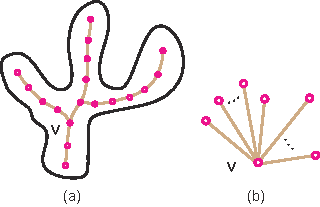
\includegraphics[width=0.6\linewidth]{figs/fork.png}
  \caption{\label{fig:fork}%
           A skeleton $S$ that is a fork originated from a node.}
\end{figure}

Now we claim that there is a clique cover in $G$ of size $K$ if and only if there is a skeleton partition of $S$ into $K$ support-free subgraphs(the angle between each pair of arcs is no larger than $2\theta$).
For if there is clique cover in $G$ of size $K$, then each clique in $G$ corresponds to a rooted subgraph of $S$ that satisfies the angle constraint. Conversely, if $S$ is partitioned into $K$ support-free subgraphs, then every pair of arcs in each subgraph satisfy the angle constraint, by the mapping relation, their corresponding nodes in $G$ form a clique. This completes the proof. \qed

This tells the difficulty of solving the problem of partitioning a 3D model into the least number of support free pieces. In the following, we shall show how to solve the problem with a practical yet efficient algorithm.

However, as the topology of the skeleton $S$ is a tree such that the degree of each node of the tree is no larger than a constant $d$, and the least number of support-free subgraphs is bounded by another constant $c$, then we show that the problem of partitioning $S$ into the least number of support-free subgraphs (satisfying the angle constraint) can be computed in polynomial time. In general, for a tree structure with arbitrary $c$ and $d$, we have them following theorem.

\emph{\textbf{Theorem 2}: Given three integer numbers $c$, $d$, Let $S$ be a tree structure such that the degree of each node is bounded by $d$, then whether $S$ has $c$ support-free subgraphs can be determined in $O(2^{cd}n^{2c})$ time, and a partition instance can be reported within the same time bound.}

\emph{Proof}: We shall prove the theorem by construction. In taking a subgraph from a tree structure $S$, we can duplicate a node $v$ and take a subset of arcs incident to it. Given a node with $d$ arcs incident to $v$, then the number of subsets of arcs incident to it is $C(d, 1) + C(d, 2) + ... + C(d, d-1) = O(2^d)$.
In order to construct a partition of $S$ into $c$ subgraphs, we need to choose at most $c$ nodes from $S$ (it is possible that multiple subgraphs are derived from a common node). More precisely, we need to choose $i$ nodes from $n$ nodes of $S$ for $1\leq i \leq c$. Since there are $O(2^d)$ choices for each node, the number of all possible partitions is bounded by $O(\sum_{i=1}^{c}C(n, i)*C(i*2^d, c))= O(2^{cd}n^c)$.
For the resulting partition, we need to make sure that it is a valid partition, i.e., no two arcs are contained in more than one subgraph. This can be done in $O(n)$ time by counting the total number of arcs in the resulting partition: if it is equal to $(n-1)$, then the partition is valid; else otherwise. For each valid partition, we need to determine whether a subgraph is support-free. For this purpose, in each valid partition, for a subgraph of size $n_i$, it takes $O(n_i)$ time to check whether the subgraph is a support-free one given a node as the root. Therefore it takes $O(n_i^2)$ time for processing all nodes in the subgraph. In sum, it takes $O(\sum_{i=1}^{c}n_i^2) = O(n^2)$ time to check whether a partition is a support-free one. Therefore, for all $O(2^{cd}n^c)$ partitions, it requires $O(2^{cd}n^c*n^2) = O(2^{cd}n^{2c})$ time. This completes the proof \qed

As a result, if $c$ is a constant, then partitioning $S$ into $c$ support-free subgraphs can be done in polynomial time. Further, the least number of subgraphs can be determined by a standard binary operation on $c$. More precisely, if $c$ is sufficient to obtain a feasible support-free partition, then we can try $c/2$, and then $c/2^2$ if $c/2$ is also sufficient, and so on so forth, finally, a half interval is added back, and the number before and after this resulting number are used to locate the final value of the smallest number. The construction process in the proof of Theorem 1 directly suggests a polynomial time algorithm for computing the least number of support-free subgraphs when $S$ is a tree structure with constant $c$ and $d$.}}

A general graph $G$ (not necessarily a tree) can be decomposed by taking a node and a subset of arcs incident to that node, a feasible subgraph can also be a graph with cycles in it. However, splitting a node on a cycle of $G$ cannot split $G$ into two disjoint components. Next we consider the case when each subgraph is a tree structure: If the genus (number of handles) of a model is $h$ , then its corresponding skeleton contains $h$ cycles, where $h$ can be determined by the Euler formula on 3D mesh models; it requires at least $h$ splitting nodes to split $G$ into a tree structure ( which has $C(n, c) = O(n^c)$ choices); thereafter, Theorem 2 addresses the remaining splitting issue. To summarize, we have the following theorem for a general graph $G$.

\emph{\textbf{Theorem 3}: Given three integer numbers $c$, $d$ and $h$, Let $S$ be a general graph with a genus of $h$ such that the degree of each node is bounded by $d$, then whether $S$ has $c$ support-free subgraphs can be determined in $O(2^{cd}n^{2c+h})$ time, and a partition instance can be reported within the same time bound.}

We formulate the partition problem with the objectives of both the total number of cuts and the cutting length, under the constraint of printing angle of each branch with respect to the build platform, the angle between a cutting plane and the printing direction, the dimension of each printed model with respect to the printable volume of a given printer, and the base area of a printed model. Since the problem is NP-hard, we propose a randomized Monte Carlo method in compliance with a set of carefully designed selection strategy to seek a practical solution. Figure \ref{fig:ex1} shows an example of a deer model (shell), our partition result based on Laplacian skeleton of the model, the printing result and the assembly effect. The details of Monte Carlo method is given below.




%-------------------------------------------------------------------------
\section{Algorithm}
%\textbf{Skeleton Partition.}
Let $M$ denote the mesh model, and let S denote the Laplacian skeleton obtained via the algorithm provided in \cite{AuTCCL08}. We propose an algorithm for partitioning $M$ into a minimum set of \emph{disjoint} components, each of which can be fabricated in a 3D printer without using any support structure. Decomposing $S$ into two pieces can be done by duplicating a node $v$; while partitioning $M$ at node $v$ requires the determination of the position and normal of a cutting plane. To guarantee an aesthetical look on the resulting surface with shortest seams, we need a constraint to minimize the peripheral length of the cut in terms of the position and normal of the cutting plane. Note that the orientation of the cutting plane affects the printing direction and thus the shape of the subgraph while on the contrary, the shape of the subgraph constrains the orientation of the cutting plane. Hence, this is an essential \emph{chicken-and-egg} problem. In addition, we also need to consider the printing volume limit, i.e., the volume of the printing model should be within the working volume of a given 3{D} printer.

To summarize, our objectives are the minimization of: (1) the number of partitioned components $N$ of the mesh model; (2) the total peripheral length of each cut $L_i$, i.e., $\Sigma L_i$. The constraints of the problem are as follows:


(i) Each arc of the partitioned subgraph $H_i$ subtends to an axis by an angle of no larger than $\theta$, where $\theta$ is a printer-dependent parameter obtained from experiments. This guarantees that the corresponding mesh component is support-free during the printing process;


(ii) As the directed arcs of $H_i$ are translated to a common origin, they form a fork (see Figure \ref{fig:cone}). Let $a$ and $b$ be the pair of farthest vectors in the fork, i.e., the angle between $a$ and $b$, denoted as $\alpha$, is the largest. Let the central ray of the minimum cone that encloses the fork be denoted as $r(H_i)$, then $r(H_i)$ is collinear with $a + b$. Then the feasible directions of printing $H_i$ without using any support is bounded by a solid cone centered at $r(H_i)$ with an apex angle of $2\theta - \alpha$ (Figure \ref{fig:cone}). Therefore, let $b(H_i)$ be the base cut of the mesh part that corresponds to the root of $H_i$ {(by base cut we mean the cutting boundary which adheres to the printing platform when the part is being printed, see Figure \ref{fig:ex1} (d))}, then $b(H_i)$ is orthogonal to some vector $\hat{e}$ in $cone(H_i)$. %This guarantees that the base can be placed on the 3D printing platform.

Thereafter, in order to guarantee support-free fabrication of any cut other than the base, the angle between any non-base cut and the base cut should be no larger than $\theta$ since the base cut determines the printing direction. More precisely, any other cut $c$ separating subgraph $H_i$ from another subgraph $H_j$ should satisfy the constraint that the angle between $c$ and $b(H_i)$ is no larger than $\theta$. Let $A(c, b(H_i))$ denote the angle, then $A(c, b(H_i)) \leq \theta$. Since a cut separates the mesh into two parts, possibly sacrificing the angle constraint of the mesh part corresponding to a subgraph adjacent to $H_i$, an additional cut respecting the angle constraint of the adjacent subgraph may be required. Detailed steps for addressing this issue is given in the section for Mesh Partition below.

\begin{figure}[t]
  \centering
  \includegraphics[width=0.7\linewidth]{figs/cone.png}
  \caption{\label{fig:cone}%
           Illustration of $r(H_i)$ and $cone(H_i)$.}
\end{figure}

%As a cut partitions a shell model, one facet is generated for the CAD model, but it two facets are generated physically, . Let the normal direction of the cut $c$ (pointing to the exterior of the partitioned part) be denoted as $n(c)$.

%Mathematically, a cut behaves as a single facet for the mesh; but it results in two facets on the appearance of the physical model. With the physical understanding, for each cut c, let $c_1$ and $c_2$ be the two facets on the physical model. Since $M$ is a shell mode, $c_1$ and $c_2$ are two annular-shaped plane facets. Let $n(c_1)$ be the normal direction of $c_1$ that points into the interior of the shell. $n(c_1)$ is defined similarly.


(iii) The base of a printing model should be large enough to gather sticky force from the building platform, such that the model is not deformed during the building process. Formally, let $area(b(H_i))$ denote the area of the base of the mesh component corresponding to $H_i$, which is approximately equal to the peripheral length of the base times the thickness of the shell. let $\tau$ be a user-defined threshold value, then we have $b(H_i) \geq \tau$. Here $\tau$ can be determined empirically; Finally,


(iv) Each cut partitions a single subgraph.

We have the following optimization system:
\begin{equation*}
\begin{aligned}
& \underset{x}{\text{minimize}} \quad N \quad \text{and} \quad \sum_{i=1}^N{L_i},
\quad \text{subject to:} \\
& A(e, r(H_i)) \leq \theta, \; i = 1, \ldots, m, \forall e \in H_i, & (1)\\
& b(H_i) \bot \hat{e}, \hat{e} \in cone(H_i), & (2)\\
& A(c, b(H_i)) \leq \theta, & (3)\\
& area(b(H_i)) \geq \tau, & (4)\\
& cut \cap S = cut \cap H_i, cut \in \{b(H_i), c\}  & (5)
\end{aligned}
\end{equation*}
where all $H_i$-s constitute a partition of the original graph. A direct exploration of all possible partitions over the graph $G$ could quickly leads to exponential complexity. The key here is to quickly find potential good partitions in a way that subsequent exploration of the graph is limited to those which leads to a less value of the optimization function. We employ a randomized Monte Carlo algorithm detailed below.

We separate the minimization of the two target terms sequentially, i.e., the number of mesh components and the total cutting length. In the following, we shall discuss how the skeleton and mesh are partitioned in details.

\textbf{Skeleton Partition.} To minimize the number of subgraphs,
we use a randomized exploration strategy, but give a higher probability to explore the graph broadly. In particular, assume that we are given a function $Trim\_BFS(v, G, \theta)$ which traverses $G$ from $v$ in a breath first search manner to progressively collect arcs which satisfy Constraint (1); and a function $MeshPartition(U , M)$ that decomposes $M$ based on the set of partitioned subgraphs $U$, and returns a partition of $M$, denoted as $M^{'}$, and the number of cuts $N$. Algorithm \ref{alg:Framwork} sketches the idea of the skeleton decomposition. The main idea is to randomly search for candidate subgraphs using Monte Carlo Method, which randomly chooses a node of $G$ to start traversing and randomly grows the subgraph while paying attention to the aforementioned constraints.

\begin{algorithm}
\caption{$Skeleton\_Mesh\_Decomposition(S, M)$}
\label{alg:Framwork}
\begin{algorithmic}[1]
\REQUIRE~
The Laplacian skeleton $S$ and mesh model $M$.
\ENSURE~
The decomposition of $M$ into the least pieces of components that are free of support.

%; a partition of $M$ based on $T$ that satisfies constraint (2-4)
\STATE $M_{opt} = \emptyset$; $min = \inf$; $count$ = 0; $max\_iter$ = a user defined large constant;
\WHILE {$count < max\_iter$}
\STATE  $U= \emptyset$;
\WHILE {$S\neq \emptyset$}
\FOR{$i=1$; $i<|| S ||$; $i++$ }
\STATE $H = Trim\_BFS(v_i, S, \theta)$;
\STATE $S = S / H$;
\STATE $U = U \cup H$;
\ENDFOR
\STATE $(M^{'}, N) = MeshPartition(U , M)$;
\IF {$N < min$}
\STATE  $min = N$;
\STATE  $M_{opt} = M^{'}$;
\ENDIF
\ENDWHILE
\STATE $count =count + 1$;
\ENDWHILE
\RETURN  $M_{opt}$;
\label{code:fram:select} \\
%\STATE call function $Mesh\_Decomposition(M, T)$;
\end{algorithmic}
\end{algorithm}




\begin{figure}[tbp]
  \centering
  \includegraphics[width=\linewidth]{figs/take_arc.png}
  \caption{\label{fig:sphere}%
           Illustration of unit vectors, unit sphere, spherical disks, and the determination of taking a new edge in $Trim\_BFS$.}
\end{figure}

Next we shall show how $Trim\_BFS(v, G, \theta)$ works to find a locally maximal subgraph starting at $v$ that satisfies the angle constraint. Let $H$ be the current subgraph obtained so far. When an arc $e$ of $G$ is visited, we need to determine whether it should be included into $H$. If the start of each outgoing arc of $H$ is moved to a common origin, then the arcs form a fork of rays (Figure \ref{fig:sphere}). A naive method to judge whether $e$ should be included is to move the start of $e$ to the origin of the fork, and compute the angle between $e$ and each arc of the fork, $e$ is included if the maximum angle between $e$ and each arc of the fork does not exceed 2$\theta$. However, this would lead to $O(n^{2})$ time complexity of $Trim\_BFS(v, G, \theta)$, where $n$ is the size of $G$. To speed up this process, we keep the pair of vectors which form the largest angle and judge whether a new vector expands the angle of the fork. See Figure \ref{fig:sphere}, let $\hat{e_i}$  and $\hat{e_j}$ be the units of these two vectors obtained so far. For simplicity, we denoted by $F( \hat{e_i}, \hat{e_j} )$ the fork with the starts of all unit vectors converging at the origin of the coordinate frame, where $\hat{e_i}$  and  $\hat{e_j}$  are the pair of unit vectors that form the largest angle in the fork. Let $\hat{e_k}$  be the unit of a new vector to be processed next, if $\hat{e_k}$ penetrates through the blue circle, then no change need to be made to the fork; otherwise, let $D_{i,j}$ denote the spherical disk that passes through the endpoints of $\hat{e_i}$  and $\hat{e_j}$ whose central axis is collinear with $\hat{e_i}$  + $\hat{e_j}$, let $c_{i,j}$ be the center of $D_{i,j}$, let $B_{i,j}$ be the boundary circle of $D_{i,j}$. The circle passing through $\hat{e_k}$  and $c_{i,j}$, denoted as $O( \hat{e_k}, c_{i,j})$, intersects  $B_{i,j}$ at two points, let $q$ the point further away from the endpoint of $\hat{e_k}$, then $\overrightarrow{oq}$ and $\hat{e_k}$ are the two extreme vectors that to be used in the next iteration. To summarize, a new arc $e_k$ is taken by $Trim\_BFS$ if and only if one of the following two conditions is met:
(1) the angle between $\overrightarrow{oc_{i,j}}$ and $\hat{e_k}$, denoted as $A(\overrightarrow{oc_{i,j}}, \hat{e_k})$, satisfies  $A(\overrightarrow{oc_{i,j}}, \hat{e_k}) \leq A(\overrightarrow{oc_{i,j}}, \hat{e_i})$;
(2) $A(\overrightarrow{oq}, \hat{e_k})  \leq  2\theta$, where $q = O( \hat{e_k}, c_{i,j}) \cap B_{i,j}$.


\begin{algorithm}[t]
\caption{Algorithm: $Trim\_BFS(v, S,\theta)$}
\label{alg:trim}
\begin{algorithmic}[1]
\REQUIRE~
A node $v$ of Laplacian skeleton $S$, an angular value $\theta$.
\ENSURE~
 %A maximal subgraph $H$ rooted at $v$ and its corresponding mesh component that meet the constraints $(Eq.1-4)$.
 A subgraph $H$ rooted at $v$ that meets constraint (1).
\STATE starting from $v$, initialize F($\hat{e_i}$, $\hat{e_j}$); $H = \emptyset $;
\WHILE  {the current arc $e_k$ of $S$ picked by the BFS process is nonempty}
  \IF  {$A(\overrightarrow{oc_{i,j}},  \hat{e_k}) \leq A(\overrightarrow{oc_{i,j}},  \hat{e_i})$}
  \STATE  $H = H \cup \{e_k\}$;
  \ELSIF {$A(\overrightarrow{oq},  \hat{e_k}) \leq  2\theta$}
  \STATE $q = O( \hat{e_k}, c_{i,j}) \cap B_{i,j}$;
%  \IF  {$A(\overrightarrow{oq},  \hat{e_k}) \leq \pi- 2\theta$}
  \STATE  $\hat{e_i}=  \hat{e_k}$;
  \STATE $\hat{e_j} =  \overrightarrow{oq}$;
  \STATE  update $B_{i,j}$ and $c_{i,j}$;
  \STATE  $H = H \cup \{e_k\}$;
  \ENDIF
\ENDWHILE
%\STATE  call the cutting scheme for $M$;
%\STATE  $M= M/M_H$;
\label{code:fram:select} \\
%\RETURN  $H$ and $M_H$;
\RETURN  $H$;
\end{algorithmic}
\end{algorithm}

Algorithm \ref{alg:trim} demonstrates the growing process. Since the order of the chosen arcs influences the shape of the final BFS subgraph, in line $2$, the BFS process randomly chooses an arc incident to $v$ to proceed on. In order to guarantee a greater chance of converging to the optimal result in a short time, we refine Algorithm \ref{alg:trim} by inducing probabilities of choosing each arc of $S$. We denote this improved version of Algorithm \ref{alg:trim} as \textbf{$Trim\_BFS\_II$}. The main idea of $Trim\_BFS\_II$ is as follows.
We apply a training-and-learning procedure for the first $k$ (say $1000$) runs. Formally, let $n_v$ be the number of times an arc is chosen as the exit arc when node $v$ is visited. Given the data of the first $k$ runs, when a node $v$ is visited, the probability of choosing an arc $e$ as an outgoing arc in the subsequent runs is, $P(v, e) = n_v/k$.

%To further speed up the process of $Trim\_BFS$, we assign a mark that stores the minimum number of subgraphs obtained so far, such that the current branching can be terminated if its output number of subgraphs is larger than the mark.


Further, as $Trim\_BFS\_II$ is greedy, the growth is towards a local maximal subgraph that satisfies the angle constraints, the resulting partition of Algorithm \ref{alg:Framwork} might not be a global optimum. In order to ensure more possibilities to find a global optimum, we set a probability-based scheme to terminate the growing of a subgraph. The probability to terminate the growing is set to $r/n$, where $r$ is the size of the current subgraph and $n$ is the size of $G$. This gives high probability for $Trim\_BFS\_II$ to grow in larger sizes while rising the probability of exploring subgraphs of smaller sizes. We implemented it using rejection sampling.

%Since the traversing process assigns a specific direction to each arc that was originally undirected in $S$, it is not obvious whether the angle constraint is satisfied, To clarify this, we provide the following lemma.


%\begin{figure}[t]
%  \centering
%  \mbox{} \hfill
%  \includegraphics[width=0.4\textwidth]{figs/proof.png}
%  \caption{\label{fig:proof}%
%           Illustration of taking a directed arc into a maximal subgraph by $Trim\_BFS$.}
%\end{figure}



%\emph{Lemma 1}: $H = Trim\_BFS(v, G, \theta)$ is a maximal subgraph of $G$ that satisfies the angle constraint, i.e., each arc of $H$ subtends to an axis by an angle of no larger than $\theta$.


%\emph{Proof}: Suppose to the contrary that $H$ violates the angle constraint, there exists a directed arc that does not satisfy the angle constraint. For example, arc $\overrightarrow{ca}$ or arc $\overrightarrow{bc}$ in Figure \ref{fig:proof}. Such case is impossible as Line $3$ and Line $6$ of function $Trim\_BFS$ excludes any directed arc that violates the angle constraint of no larger than $\theta$ with respect to the (virtual) central axis.It remains to prove that $H$ is maximal, i.e., the largest graph rooted at $v$ that covers all the arcs that satisfies the angle constraint. Suppose that this is not true, there must exist an arc that was mistakenly discarded due to the direction in which the arc is traversed. Let $(b, c)$ be one of such arcs, as illustrated in Figure \ref{fig:proof}(a). When the arc is directed from $b$ to $c$, it is not included as it violates the angle constraint, but can be included if the arc directed from $c$ to $b$. We shall prove in a case-by-case basis. If $c$ is not reachable from $v$ via a directed path passing through $b$ (Figure \ref{fig:proof} (c)), then $c$ is only reachable from $b$, arc $bc$ should not be included and line 6 of Function $Trim\_BFS$ correctly handle this case. Otherwise, $c$ is reachable from $v$ via a directed path without passing through $b$ (Figure \ref{fig:proof} (d)). As $c$ is visited, by Line 2 of Function $Trim\_BFS$, each arc leaving $c$ is considered, and $\overrightarrow{cb}$ is correctly included into $H$. This completes the proof.



\begin{figure}[t]
  \centering
  \includegraphics[width=0.3\textwidth]{figs/cone-fillet.png}
  \caption{\label{fig:fillets}%
           Illustration of a cone and its corresponding fillets, where two cutting planes in $F(H_i)$ and their associated vectors in $cone(H_i)$ are marked by distinct colors.}
\end{figure}


\textbf{Mesh Partition.}
{In the following section, we shall describe how MeshPartition(U , M) works as a cut is required around a skeleton node $v$. Codes are ommitted for brevity.}
The skeleton partition returns a set of nodes where the mesh partition should occur, in particular, the cutting plane should be in the vicinity of each node $v$ incident to at least two distinct subgraphs. We need to determine the exact positions and orientations of the cutting planes. For each node $v$ that is incident to at least two distinct subgraphs $H_i$ and $H_j$, we process it using the following cutting scheme.


Refer to Figure \ref{fig:fillets}, at the position of node $v$, we want to find a surface vertex $q \in M$ around $v$ through which the cutting plane should pass, while the cutting length is minimized. Let us denote the set of all planes which pass through a surface vertex $p$ and are orthogonal to vectors in $cone(H_i)$ (originated from $p$)  as $F(H_i)$, which we term as a \emph{fillet}. Then if the node $v$ is incident to two subgraphs $H_i$ and $H_j$, we have two plane sets $F(H_i)$ and $F(H_j)$ at point $p$, respectively. Depending on the position of $p$, we have the following two cases. \emph{Case (i)}: $F(H_i) \cap F(H_j) \neq \emptyset$. In this case, we shall randomly sample a set of cutting planes from $F(H_i) \cap F(H_j)$, and determine the one achieving the minimum cutting length; \emph{Case (ii):} $F(H_i) \cap F(H_j) = \emptyset$. In this case, two cuts are required in order to separate the mesh into support-free subparts. However, care must be taken as the angle between $c_1$ and $c_2$ should be constrained by $A(c_1, c_2) \leq \theta$. If this constraint is violated, one more cut in between $c_1$ and $c_2$ is required; while the base of each partitioned component should be no less than $\tau$. If any of the constraint is not satisfied, we shall translate the fillets along the printing direction in an opposite sense until the constraints are satisfied.

\begin{figure}[tbp]
  \centering
  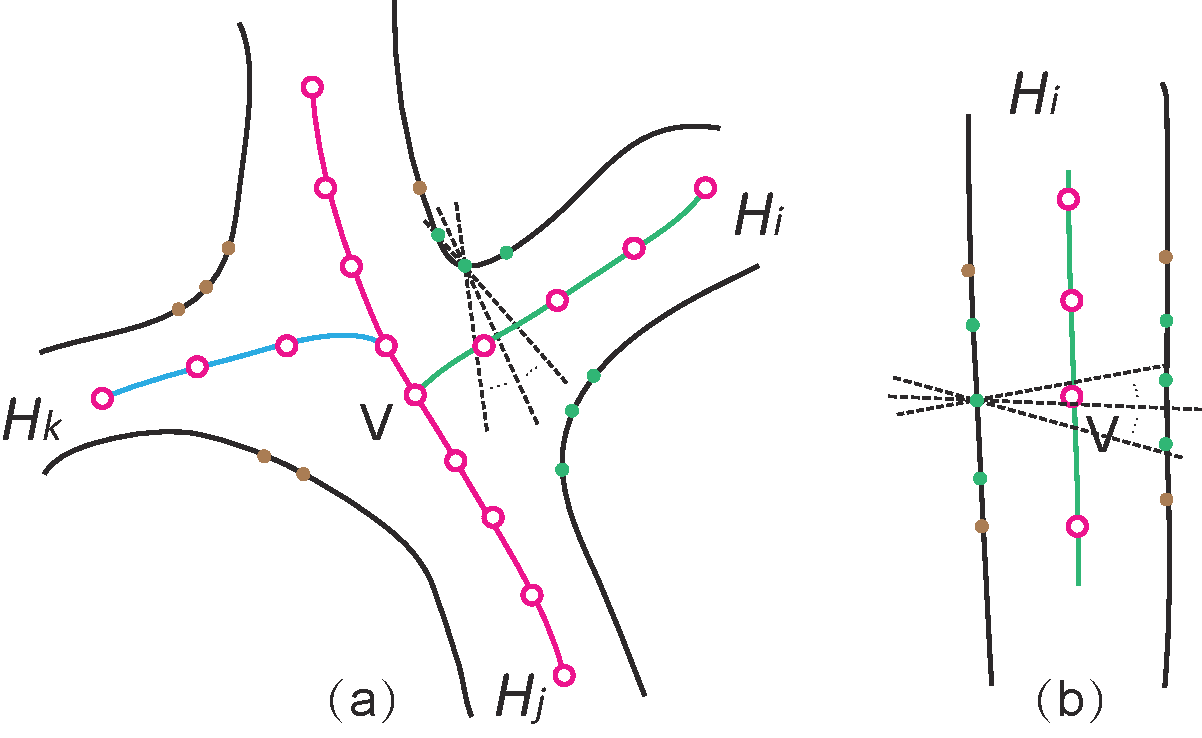
\includegraphics[width=0.4\textwidth]{figs/forward_tracing.png}
  \caption{\label{fig:forward_tracing}%
           2D illustration of R(v) and the cuts, all vertices in $R(v)$ are shown in green, and the cuts associated with a vertex are shown in dashed lines:(a) the case of cuts around concave points; (b) the case of cuts on a cylindrical part.}
\end{figure}

In either case, a cut that nicely follows the geometry features is demanded in order to preserve aesthetic appearance in the final assembled object. We exploit shape concavity to look for a good cut as indicated by minima rule \cite{hoffman1984parts,hoffman1997salience}. However, the positions of the skeleton nodes may not locally reflect the geometric features such as concave areas on the mesh surface, therefore they are insufficient for a nice partition of the mesh. To compensate this, we exploit the concave vertices of the mesh that are incident to the skeleton nodes and take those that significantly concave into a candidate set of pivots for the cuts. More precisely, let $R(v)$ be the set of concave vertices on $M$ that are incident to $v$ during the Laplacian shrinking process \cite{AuTCCL08}, we truncate $R(v)$ such that the insignificant concave vertices are removed away. Here, given a vertex $v_i$ and any of its neighbor $v_j$, $v_i$ is concave if $(v_i - v_j)(n_j - n_i)$ is nonnegative, the significance of a concave vertex can be quantified as the magnitude of $(v_i - v_j)(n_j - n_i)$ \cite{au2012mesh}, denoted as $\tau_i$. We collect vertices whose $\tau_i$ is greater than a threshold $\delta$.

%See Figure \ref{fig:fillets}(c-d), for each vertex in $R(v)$, we shall process a pair of fillets as done for vertex $p$ above.


Next, we proceed to find a cutting plane around $v$. We first extend the region $R(v)$ by merging each $R(u)$ into it, where $u$ is an adjacent node of $v$ in $S$. Given all concave vertices in the new $R(v)$, each vertex defines a set of feasible cutting planes in accordance to its $fillet$. By feasible we require that a cutting plane does not cut through any other subgraph except for $H_i$. We then exhaustively go through all feasible cutting planes and find the one whose cutting length is minimum. In case of a cylindrical part that does not merit good concaveness, we reduce the threshold value $\delta$ by half and repeat the procedure until a feasible cutting plane with minimum length is found. Figure \ref{fig:forward_tracing} illustrates the process.


%Particularly, if $v$ is a leaf node that is merely neighbored to a single node $w$ in subgraph $H_i$, then the separation of the mesh component corresponding to $H_i$ may not be feasible if merely $R(v)$ is used, this is because the position of $v$ is chosen irrespective of the geometric features of the mesh. To separate the mesh component of $H_i$, we process arc $vw$ as follows: Given a user-defined threshold value $\delta$, if $| vw | \leq \delta$, then $R(v)$ is extended to contain the concave vertices of $M$ that are incident to $w$. On the other hand, if $| vw | > \delta$, then a partition of the arc $vw$ by an interval of $\delta$ is carried out. Subsequently, for each node along arc $vw$, the above scheme for processing node $v$ is exploited, see Figure \ref{fig:forward_tracing}. In this process, the tracing of the nodes along $vw$ stops as a cut does not intersect into any other subgraph other than $H_i$. The technique for detecting the intersection is as follows:

In order to determine whether a cutting plane cuts through any subgraph other than $H_i$, we take advantage of the correspondence between the mesh vertices and the skeleton nodes. Since each vertex of $M$ is mapped to a single node of $S$ \cite{AuTCCL08}, as a cut goes through the mesh surface, the endpoints of the edges of $M$ that are penetrated through give us the information of the potential subgraph that is cut through. Approximately, if a cut $c$ goes into an edge whose endpoints are incident to a subgraph $H_j$, then $c$ cuts through $H_j$.

%On the other hand, if $v$ is an internal node to at least two subgraphs, see Figure \ref{fig:cross}, then a partition of one subgraph around $v$ is inevitable. The partition scheme follows from the operations on the fillets.

Sometimes, it is possible for a mesh component which is not printable free of support even though its corresponding skeleton is detected to be printable free of support. This is because the skeleton piece that shares a junction node with some other subgraph may compromise its topology locally \cite{AuTCCL08}, and therefore cannot precisely describe the local topology feature of the partitioned component. In this case, we search along the skeleton and further partition it with an additional cut. Refer to Figure \ref{fig:arm} for an illustration. Empirically, we found this rarely happened.

\begin{figure}[tbp]
  \centering
  \includegraphics[width=0.3\textwidth]{figs/arm.png}
  \caption{\label{fig:arm}%
           Illustration of a mesh component with an overhange that requires support while its corresponding skeleton is support-free}
\end{figure}

%Finally, if the cut-subgraph constraint (Eq. (5)) is violated, a sequence of iterative cutting is required.










%-------------------------------------------------------------------------
\section{Results}
[In the examples, show how the training-and-learning procedure saves running time]

We have evaluated our skeletal partition approach on a number of models, including man-made art objects and organic forms. Figures LLL show partition results, and the printed models and their experimental statistics.




[show the printed model without any cutting operation, the partitioned CAD model, the assembled printed model, the statistics on time and material saving, for all 12 models]



%-------------------------------------------------------------------------
\section{Conclusion,Limitations and Future Work}

\textbf{Conclusion:}In this paper, we present a skeleton-based approach for partitioning a shell model into parts which are free of supporting structure when fabricated. We formulate the model partition problem as a constrained graph partition problem which is particularly tailored toward fabrication. To tackle the NP-hardness of the problem, we exploit a randomized Monte Carlo method which adaptively searches for better partition results while avoiding local minima. Compared with existing partition-based methods, the advantages of our partition method are as follows:

\begin{itemize}
 \item The models are support-free, especially for the 3D printing techniques including SLA, SLM and SLS. For FDM technique, it requires a bed of support that consumes very little volume of materials.
\item The seams on the assembled model are minimized in terms of cut number and cut length.
\end{itemize}

The support-free feature of our partition approach saves a significant amount of time and printing materials both inside and outside the model of a shell model. Our method is efficient and applicable to a large set of natural and man-made models.

\textbf{Limitations and Future Work:} Our approach is devoted to shell models, it can also be applied to cutting solid models without any problem. However, our approach suffers from a few limitations: 
(1) For shell models, the thickness of the shells need to be large enough such that no serious deformation is caused during the assembling process. In this work, we restrict our focus to a uniform setting of the shell thickness whose value is determined by an error-and-trial process. A future research would be to determine the minimum shell thickness in different parts of a given model, this process requires an efficient detection of self-intersection and an experimental study of the printability according to the curvature changes of the shell model. 
(2) The strength guarantee is not elaborated in this work, a possible solution is to use the algorithm in \cite{WangWYLTTDCL13} that distributes the least amount of materials for constructing a truss frame beneath the skin. Finally, our approach may allow a cut that passes through a salience region, which may hurt the appearance of the model. We found that it is difficult to make a balance between the saliency and the minimal cutting length as well as the minimal cutting numbers. A potential future research is to take care of salience region during graph partition; particularly, as a trade-off, a spatially curved cut might be a consideration to alleviate the salience problem.
(3) Currently, we set a connected flat region as the base of the a partition model, while in some cases it is possible that multiple connected flat regions on a plane set as the bases may lead to better partition result, but the determination of how many cuts and the positions of the cuts is even more very intricate and is therefore a challenging future work.



%-------------------------------------------------------------------------

%\bibliographystyle{eg-alpha}
\bibliographystyle{eg-alpha-doi}

\bibliography{egbibsample}

%-------------------------------------------------------------------------
\newpage


\begin{figure*}[tbp]
  \centering
  \mbox{} \hfill
  % the following command controls the width of the embedded PS file
  % (relative to the width of the current column)
  \includegraphics[width=.3\linewidth]{figs/01.jpg}
  % replacing the above command with the one below will explicitly set
  % the bounding box of the PS figure to the rectangle (xl,yl),(xh,yh).
  % It will also prevent LaTeX from reading the PS file to determine
  % the bounding box (i.e., it will speed up the compilation process)
  % \includegraphics[width=.3\linewidth, bb=39 696 126 756]{sampleFig}
  \hfill
  \includegraphics[width=.3\linewidth]{figs/01.jpg}
  \hfill \mbox{}
  \caption{\label{fig:ex3}%
           For publications with color tables (i.e., publications not offering
           color throughout the paper) please \textbf{observe}:
           for the printed version -- and ONLY for the printed
           version -- color figures have to be placed in the last page.
           \newline
           For the electronic version, which will be converted to PDF before
           making it available electronically, the color images should be
           embedded within the document. Optionally, other multimedia
           material may be attached to the electronic version. }
\end{figure*}

\end{document}

